
\section{Testing on the 8-bit ALU} \label{sec:alu}
To evaluate both the usefulness and correctness of the new combinational logic visualisation methods added to Issie, an 8- bit ALU was was analysed using the added features.
The schematic diagram of this ALU can be found in Figure \ref{fig:alu8bit} in Appendix \ref{app:alu}. The inputs into the schematic have a total width of 23 bits, yielding a theoretical truth table size of over 8 million rows. The truth table is generated in under 1 second, but truncated to 1024 rows. Due to its size, and given that the exact specification of the ALU was not known at that point, the numeric truth table was not massively useful. However, had the specification been known prior to analysis, the numeric truth table would have undoubtedly been useful for checking the correctness of multiple input/output combinations. In order to further understand the ALU functions, algebraic reduction was used. The inputs $A$, $B$, and $CIN$ were set as algebra; this reduced the truth table size from over 8 million rows to 64. The first 18 rows of this algebraic truth table can be seen in Figure \ref{fig:alutable}. The other inputs, $X$ and $F$, eventually propagate to the SEL ports of multiplexers and therefore cannot be set as algebra. However, this works out very well -- these inputs control the behaviour of the ALU, meaning that it is better for their values to stay as numbers in the truth table. For each combination of these control inputs, a different expression at the output of the ALU ($OUT$) can be observed. From the algebraic truth table, the logical function of the ALU was described using eight short statements:
\begin{enumerate}
    \item When $X = 0$ and $F = 0$, $OUT$ is the sum of A and B
    \item When $X = 0$ and $F = 2$, $OUT = A - B$
    \item When $X = 0$ and $F = 6$, $OUT = CIN + A - B$
    \item When $X = 0$ and $F = 4$, $OUT$ is the sum of A, B, and CIN
    \item When $X = 0$ and $F[0] = 1$ (i.e. F is odd), $OUT = B$
    \item When $X = 1$, $OUT = A \& B$
    \item When $X = 2$ or $X = 3$, $OUT$ is the XOR of A and B
    \item Otherwise, $OUT$ is $B$ right-shifted by 1.
\end{enumerate}

\begin{figure}
    \centering
    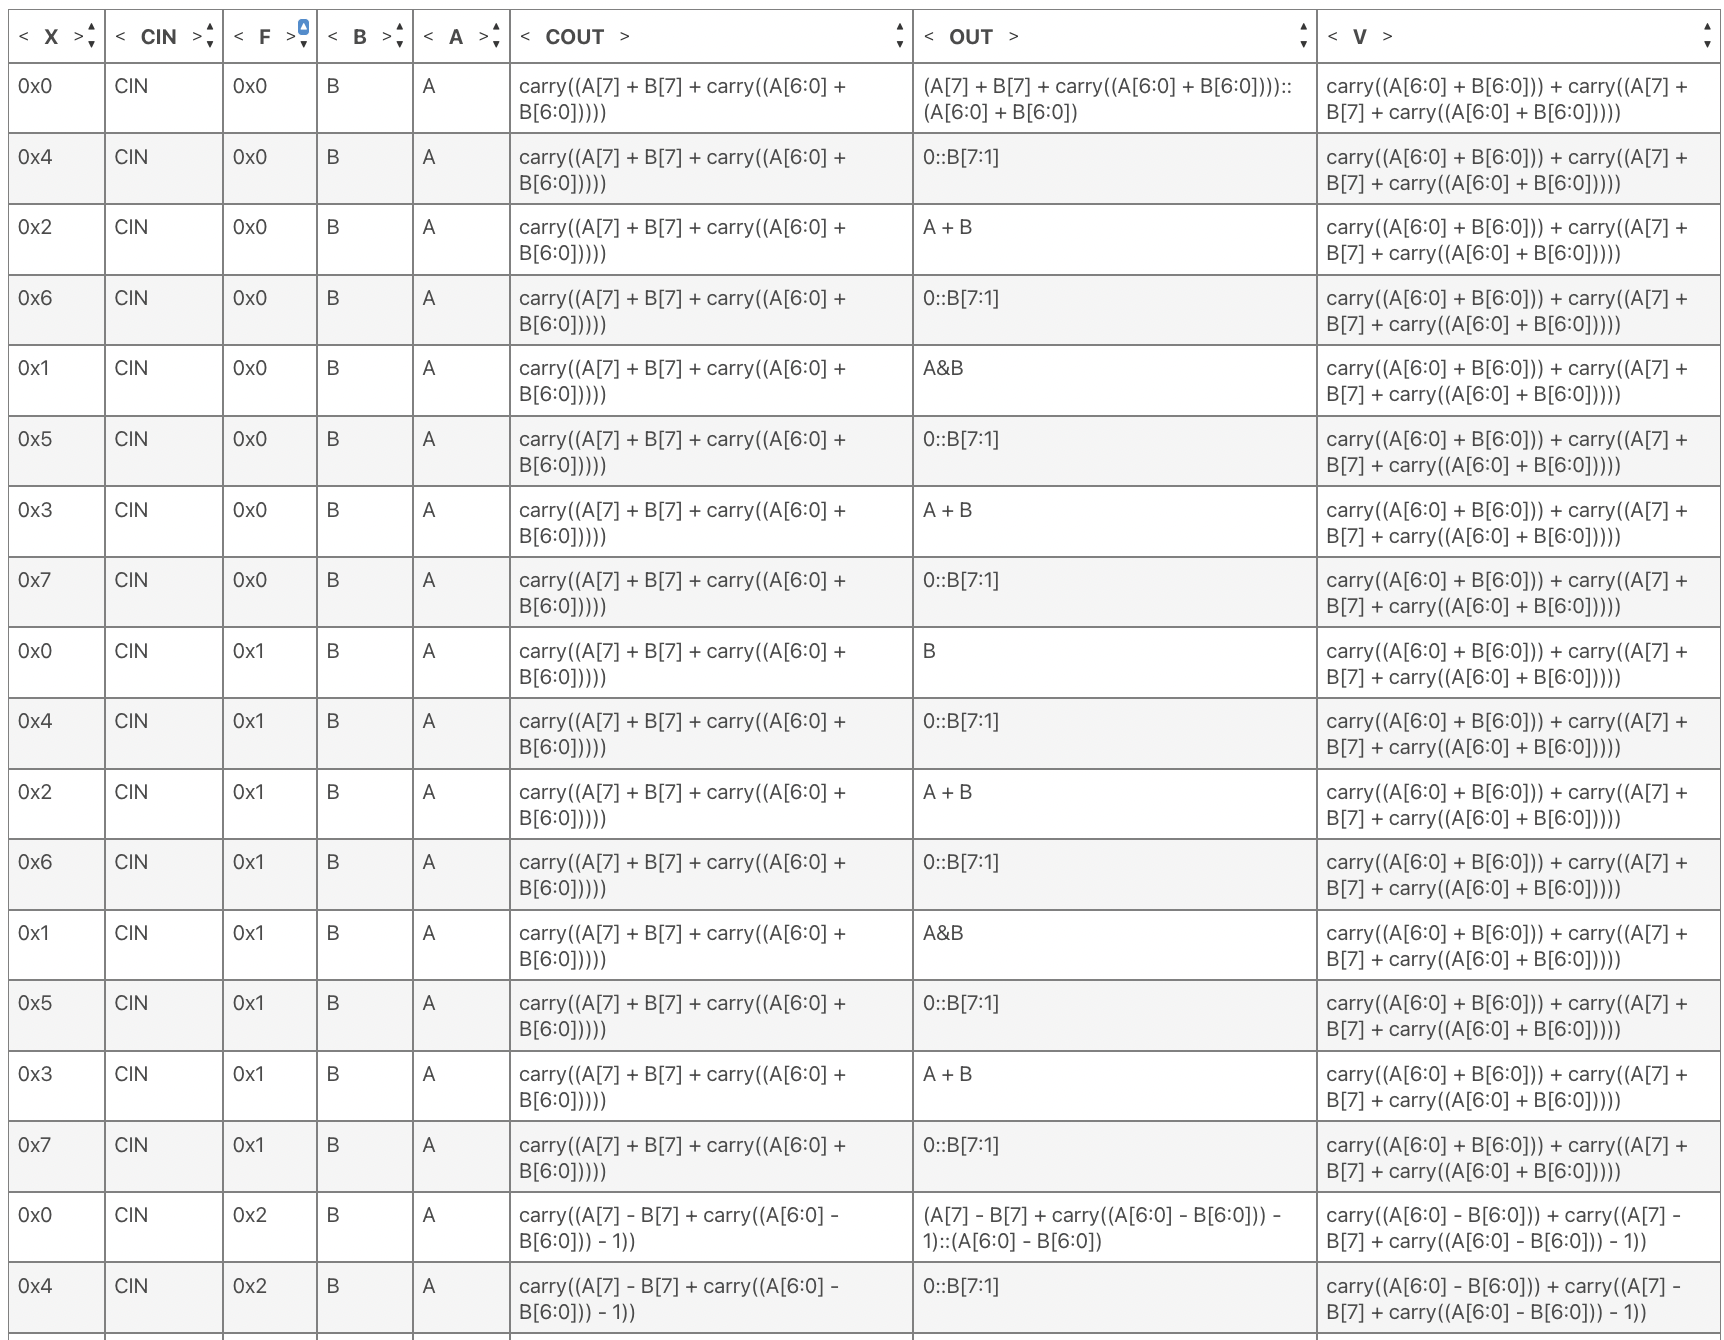
\includegraphics[width=\textwidth]{06.TestRes/alutable.png}
    \caption{First 18 rows of the Algebraic Truth Table for 8-bit ALU}
    \label{fig:alutable}
\end{figure}